\chapter{Rider control identification in bicycling under steering perturbations using a gray box approach} \label{ch:4}

\section{Methods}

\subsection{Experimental Procedure}

Twenty healthy subjects volunteered in this study. To assure safety all subjects were requested to wear protective equipment in the shape of a standards-approved bike helmet, knee and elbow pads. All participants gave informed consent according to the guidelines of the human research ethics committee of Delft University of Technology. All subjects were healthy and reported that they did not experience any kind of pain or injury in the year before the experiments. The mean weight of all subjects was selected to be close to the European population \cite{walpole2012weight}.

Each experiment trial consisted of four different speeds (i.e., 2.6, 3.7, 4.5, 5.6 \si{\meter\per s}). All experiments were performed across Heertjeslaan cycling path of TU Delft, the subjects were requested to ride the steer-by-wire bicycle in all aforementioned speeds while being  perturbed. Bilateral fixed magnitude steering torque  perturbations were applied to the upper motor of the steer-by-wire bicycle through a mobile phone interface  An additional bicycle was used from the experiment coordinator to cycle behind  the instrumented steer-by-wire bicycle and perturb the subject (see \cref{steerexperiment}). From the twenty initial participants the data of fourteen ended up being used in this study, due to hardware related malfunctions which rendered their data useless.
\begin{figure}[!h]
    \centering
    \includegraphics [width=0.6\textwidth]{images/steer_irf/steer_exp.png}
    \caption{Experimental trial performed across Heertjeslaan cycling path of TU Delft; Experiment coordinator cycling behind the steer-by-wire bicycle perturbing the subject through the mobile interface.}
    \label{steerexperiment}
    \end{figure}
\subsection{System Identification} 
The system identification procedure described in \cref{hapticFB} is also followed for this chapter. First a black box identification using the FIR model is conducted in order to  extract the linear relationship between disturbance and measurements effectively filtering intrasubject variability. This is done for both steering angle \ensuremath{\delta} and roll angle \ensuremath{\phi}. As will be later shown the intersubject variability is significant contrary to the lateral perturbation experiments. For this reason the gray box identification of the proposed rider control model is fitted on the individual responses of all participants instead of the median.
\subsubsection{Rider Control Model}
The full block diagram of the bicycle-rider system is shown in \cref{fig:intrinsic_block}. Process P consists of the bicycle dynamics given by \cref{eq:bikeEOM1,eq:bikeEOM2}. However since for this work the heading control is assumed to be insignificant, the equations of motion (EOM) are not extended with heading as an extra state. Additionally, the disturbance dynamics matrix \ensuremath{\boldsymbol{H}_d} changes in order to account for the fact that 100\% of the perturbation is transferred in the steering assembly, which means that \ensuremath{l_g=0} and \ensuremath{c_s=1}. Finally, element \ensuremath{{{M}_0}_{22}} of the mass matrix \ensuremath{\boldsymbol{M}_0} is increased by 0.21 \si{\kilogram.m^2} to account for the additional inertia induced by the passive rider \cite{schwab2012lateral}. 
\begin{figure}[h!]
    \centering
    % \captionsetup{justification=centering,margin=2cm}

    \includegraphics[width=\linewidth]{images/steer_irf/steering_block.pdf}
    \caption{Block diagram of the bicycle-rider system. System P consists of the bicycle dynamics. Controller blocks \ensuremath{K_{int}} and \ensuremath{K_{ref}} are pure gain blocks the parameters of which are estimated through gray box identification. The former works as the main reflexive controller with output the neural input \ensuremath{a}, while the latter is the intrinsic controller with output the intrinsic steering torque input \ensuremath{T^{int}_{\delta}} System \ensuremath{G_{nm}} represents the neuromuscular dynamics and its output is the reflexive steering torque input \ensuremath{T^{ref}_{\delta}}. Reflexive and intrinsic inputs combined give the complete steering torque input \ensuremath{T_\delta} to process P. All sensory inflow is delayed by \ensuremath{\tau_i} \si{\second} where \ensuremath{i} is the corresponding element of the sensory inflow vector.  }
    \label{fig:intrinsic_block}
\end{figure}
The full sensory signal vector including steering angle \ensuremath{\delta}, roll angle \ensuremath{\phi}, roll rate \ensuremath{\dot{\phi}}, steer rate \ensuremath{\dot{\delta}}, and steering torque \ensuremath{T_\delta} after being delayed by \ensuremath{\tau_i} are fed into the pure gain block \ensuremath{K_{ref}}. The produced neural input \ensuremath{a} is filtered through the neuromuscular dynamics block \ensuremath{G_{nm}} (see \cref{eq:gnmBLOCKA,eq:gnmBLOCKB}) to produce the reflexive component of the final control input to the process. As has been proven by motor control studies for the shoulder a significant part of the final forcing input is regulated through a different pathway; cocontraction \cite{schouten2008nmclab} . Cocontraction refers to the  simultaneous activation of antagonist muscles around a certain joint. This  provides the nervous system with a way to adapt the mechanical properties of the limb to changing task requirements without going through the neuromuscular lag and delay limitations of the reflexive response. In the model this is simulated by feeding \ensuremath{\delta} and \ensuremath{\dot{\delta}} to the pure gain block \ensuremath{K_{int}}.The state space representations of the aforementioned systems are discretized by zero order hold with a time step of 0.005 \si{\second}. For a look into how this time step affects simulation integration error refer to \cref{fig:convergence}. Additionally, in order to make the measured  and parametric ouptut signals comparable with simulation, they are resampled from 1000 \si{hz} to 200 \si{hz}.  For gray box identification 7 parameters in total are used. Five parameters for the five gains of \ensuremath{K_{ref}} and two parameters for the two gains of \ensuremath{K_{int}}.




The gains are estimated by fitting the model output into the non-parametric data-set by minimization of the cost function :
\begin{equation}
    V_{N}(\boldsymbol{\theta})=\frac{1}{N} \mathlarger{\mathlarger{\mathlarger{\sum}}}_{k=1}^{N}\left[0.16\frac{\left(\hat{y}^{\delta}_k(\mathbf{\theta})-y^\delta_k\right)^{2}}{\left(\overline{y}^{\delta}_k\right)^2}+0.8\frac{\left(\hat{y}^{\phi}_k(\mathbf{\theta})-y^\phi_k\right)^{2}}{\left(\overline{y}^{\phi}_k\right)^2}+0.04\frac{\left(\hat{y}^{T_\delta}_k(\mathbf{\theta})\right)^2}{\left(\overline{y}^{T_\delta}_k\right)^2}\right]
    \label{eq:cost2}
    \end{equation}


where \ensuremath{\boldsymbol{\theta}} is a vector containing all the free parameters, \ensuremath{\hat{y}^{\delta}} and \ensuremath{\hat{y}^{\phi}} are the outputs of the simulation for the measured external disturbance \ensuremath{w} and the vector of parameters  \ensuremath{\boldsymbol{\theta}} for steer angle \ensuremath{\delta} and heading angle \ensuremath{\phi}  respectively, while \ensuremath{y^\delta} and \ensuremath{y^\phi} are the outputs of the non-parametric model. inally \ensuremath{\overline{y}^{\delta}_k,\overline{y}^{\phi}_k,\overline{y}^{T_\delta}_k} are the absolute maximum allowable values of the non-parametric signals and are equal to 0.4 \si{\radian}, 0.4 \si{\radian}, 10 \si{N.m} respectively.

The first two terms  of the cost function are trying to match the steering and roll  response of the parametric model with that one of the non-parametric model, while the third on minimizes the amount of input torque generated in order to produce the best possible fit while maintaining minimal control effort. The weights are chosen heuristically. For optimization the genetic algorithm with a fitness limit of 0.03 is first  used in order to produce a good starting parameter vector for gradient descend algorithm to take over, which finally finds the closest possible estimate of the global minimum. For the genetic algorithm a crossover fraction of 0.85  along with a population size 10 times the length of the parameter vector is used. 

To assess fitting performance the \ensuremath{\mathrm{VAF}} for \ensuremath{\phi} and \ensuremath{\delta} is used as defined by \cref{eq:VAF}.
\section{Results}
\subsection{Non parametric Model}
The level of fit of the non-parametric model to the measured signals as a function of forward speed is seen in \cref{fig:FIT_FIR} for all 14 participants. The \ensuremath{\mathrm{VAF}} is significantly low for both outputs which indicates that there is significant variability of the individual rider response within the trials; especially for the lowest forward speed level. 
\begin{figure}[h!]
    \centering
    % \captionsetup{justification=centering,margin=2cm}

    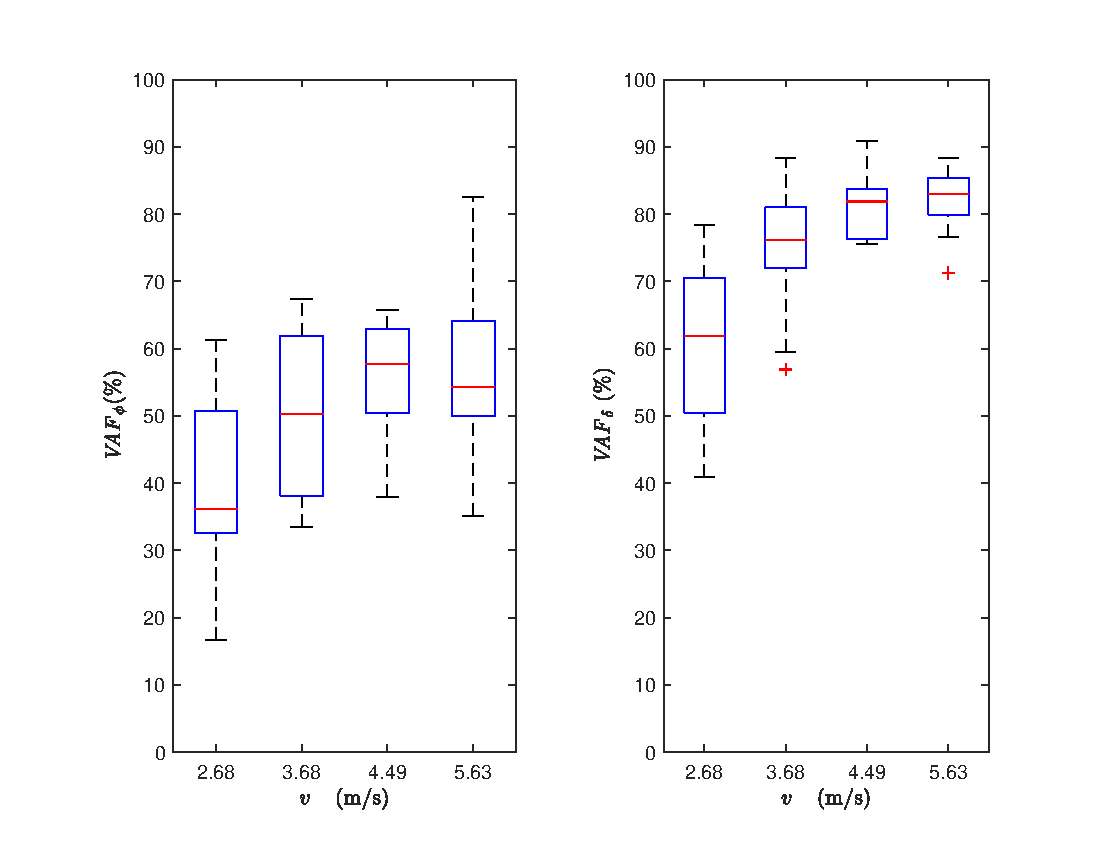
\includegraphics[width=\linewidth]{images/steer_irf/FIT_irf_steer.eps}
    \caption{Box plot of the  \ensuremath{\mathrm{VAF}} between measurements of \ensuremath{\delta} and \ensuremath{\phi} and non-parametric outputs \ensuremath{y^\delta} and \ensuremath{y^\phi} respectively for all forward speed levels.}
    \label{fig:FIT_FIR}
\end{figure}

The impulse response functions produced by fitting the FIR model into the measured data for roll and steer is seen in \cref{fig:IRF_all}. The results show great variability amongst participants.
\begin{figure}
    \centering
    \begin{subfigure}[b]{\textwidth}
        \centering
        \makebox[\textwidth][c]{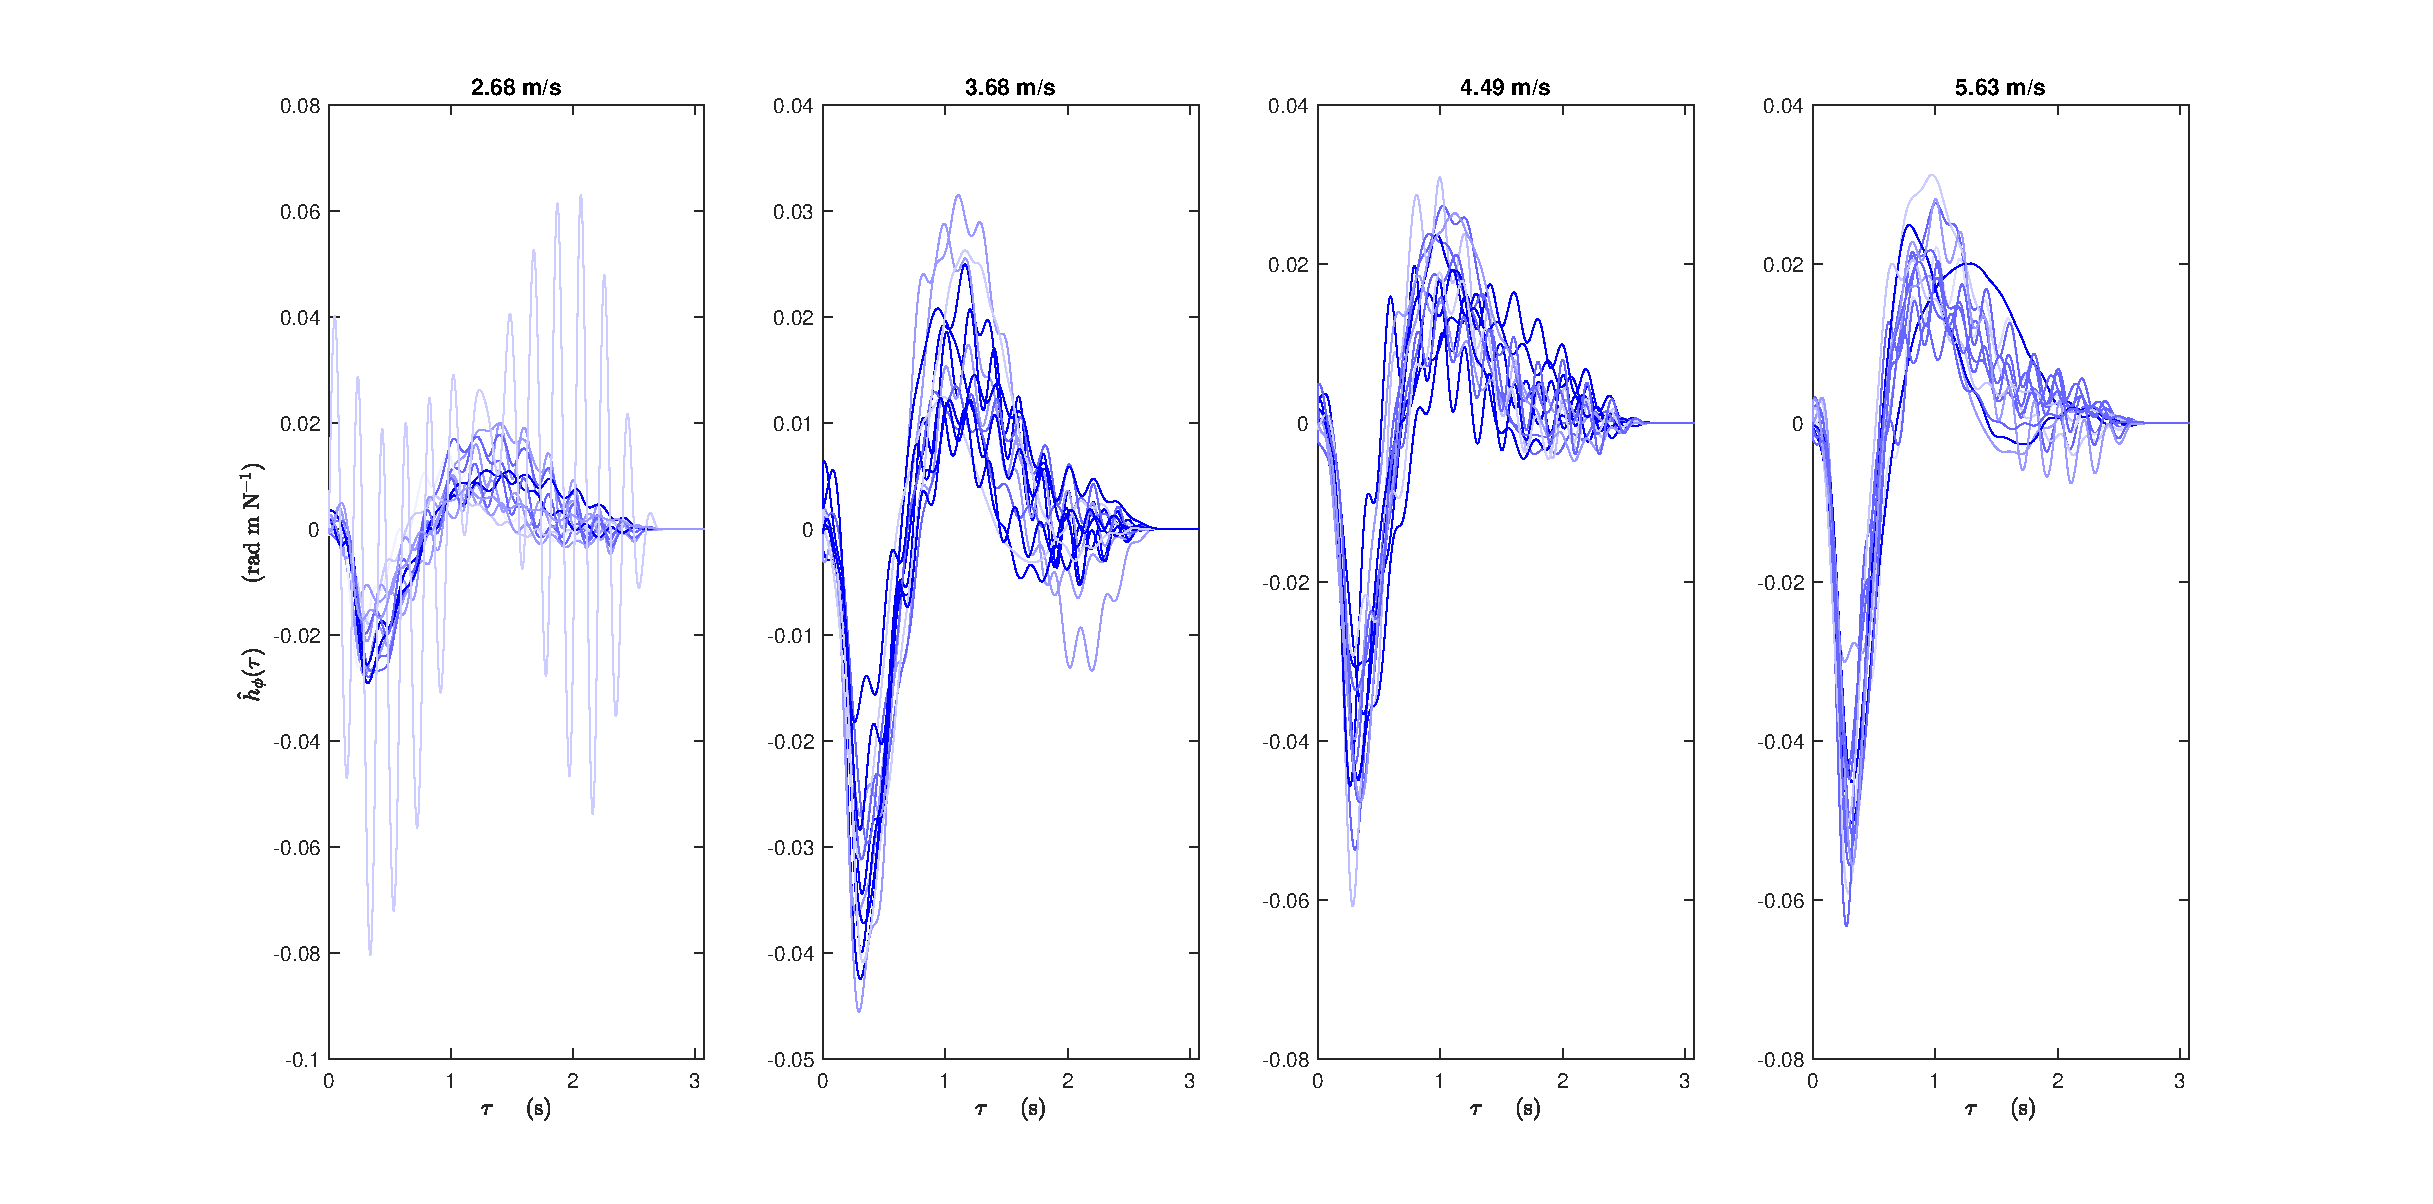
\includegraphics[width=1.1\linewidth]{images/steer_irf/roll_irf_steer.eps}}
        \caption{}
        \label{fig:IRF_phi}
    \end{subfigure}
    \begin{subfigure}[b]{\textwidth}
        \centering
        \makebox[\textwidth][c]{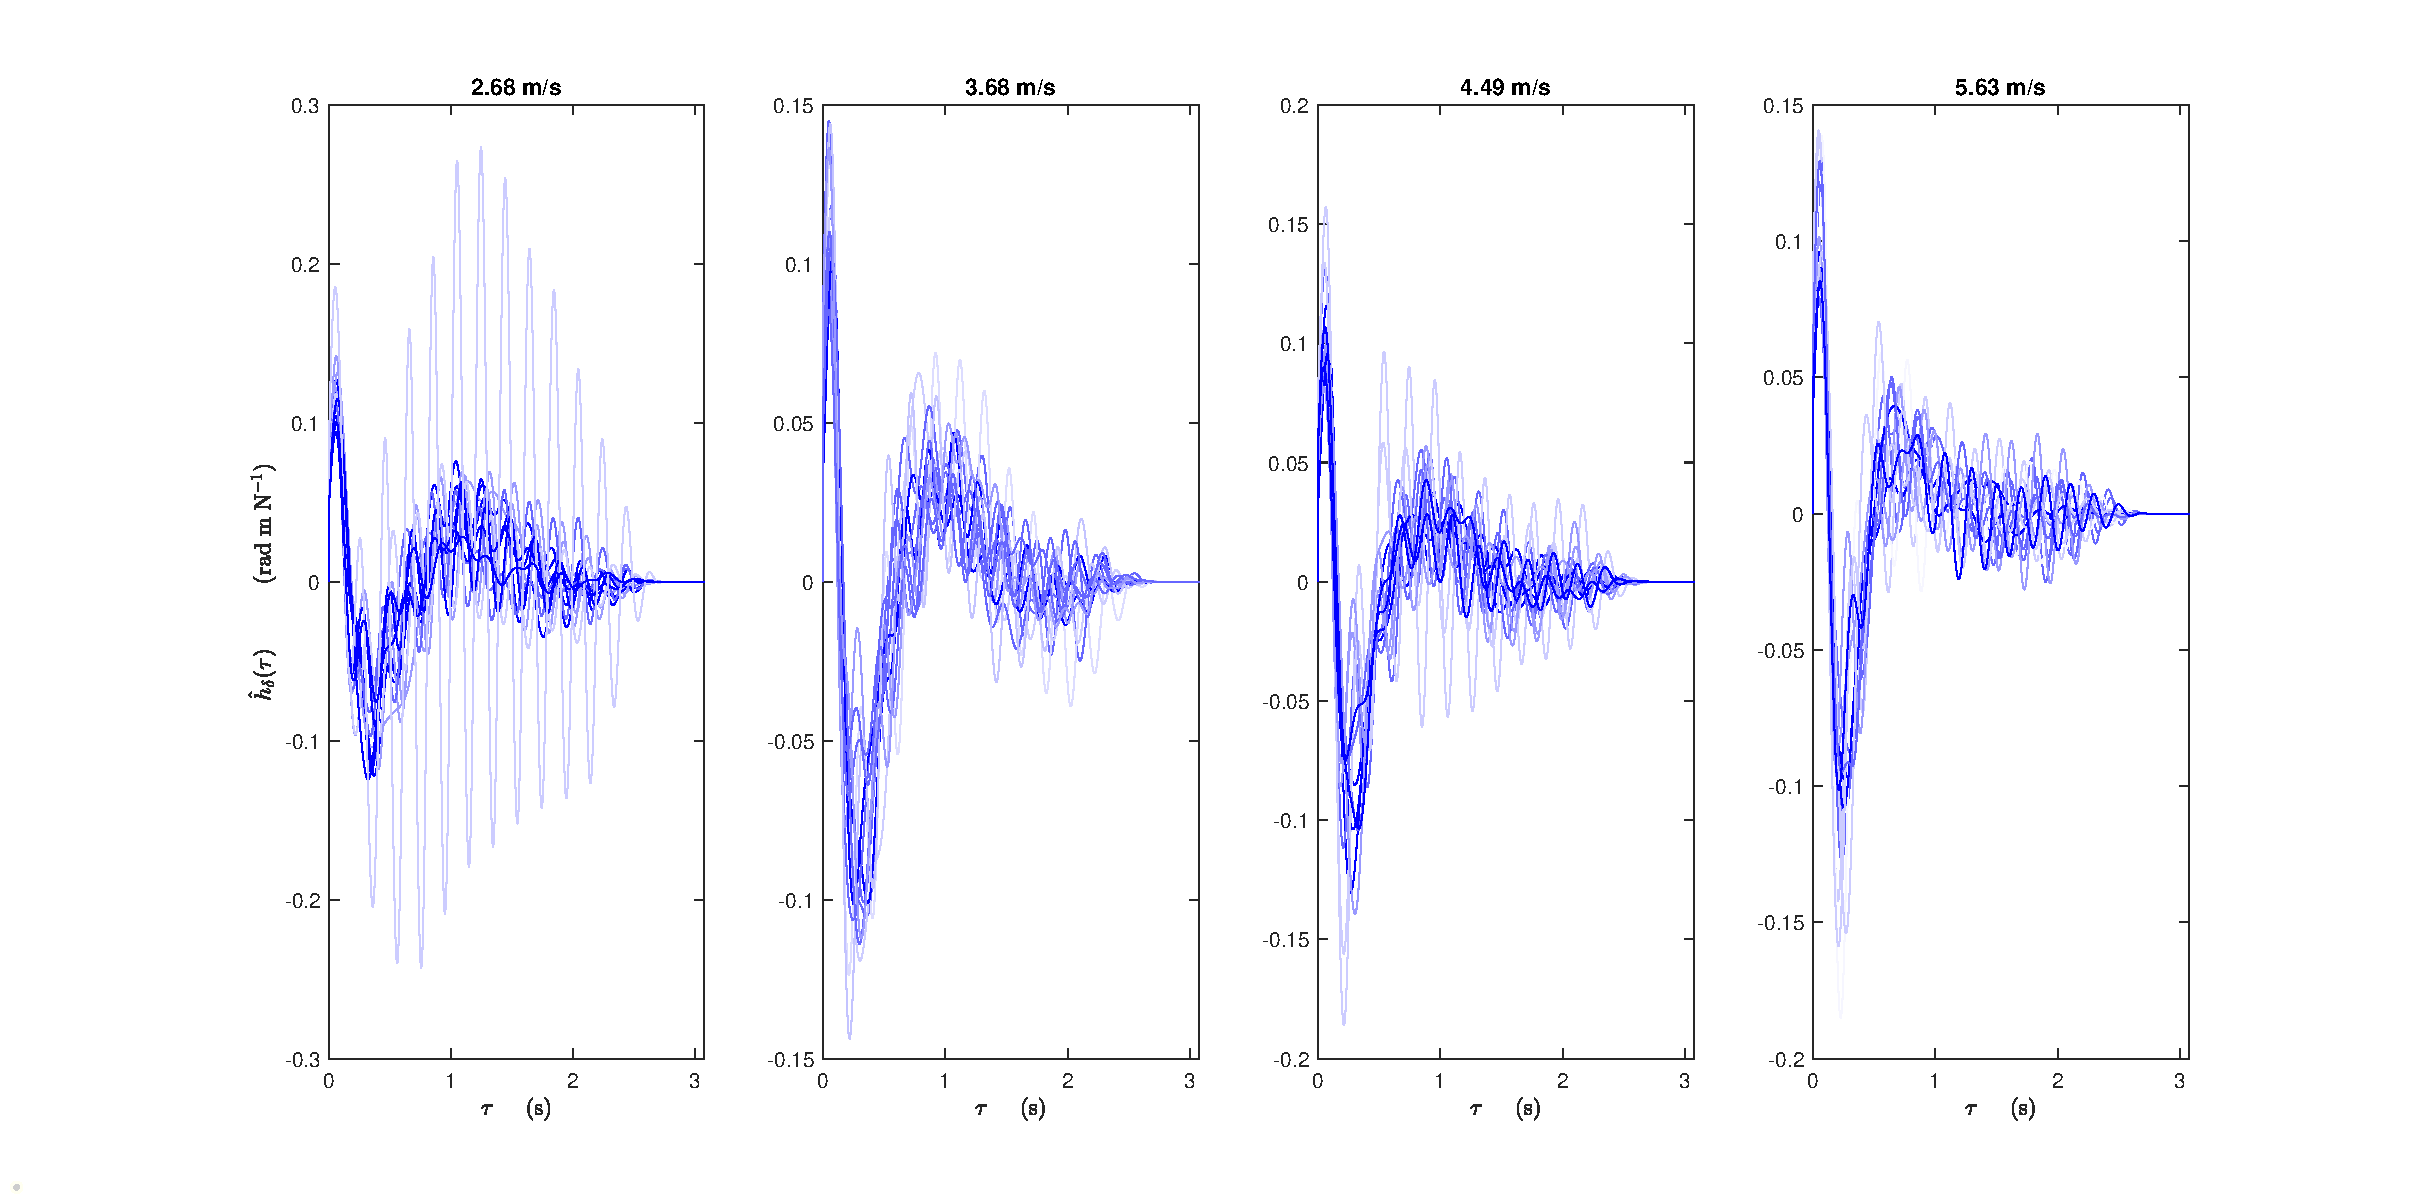
\includegraphics[width=1.1\linewidth]{images/steer_irf/steer_irf_steer.eps}}
        \caption{}            
        \label{fig:IRF_delta}
    \end{subfigure}
    \caption{Impulse response functions estimates produced by the FIR model  roll (a) and steer(b) for all forward speed levels. The closer a response is to the mean rider the more red  the lines.}
    \label{fig:IRF_all}
 \end{figure}
\subsection{Parametric Model}
The proposed rider control manages to match the non-parametric outputs with an overall good level of fit between both roll and steer (see \cref{fig:FIT_model}). The roll  shows comparatively lower fit performance but increases as forward speed gets bigger. This indicates some potential bicycle model inaccuracy which  leads to mismatch in steer-roll coupling dynamics for low speeds.   In \cref{fig:model12,fig:model34}, the response of the first participant is compared with the simulated rider model output and the results show great similarity even for the control input.
\begin{figure}
    \centering
    \begin{subfigure}[b]{\textwidth}
        \centering
        \makebox[\textwidth][c]{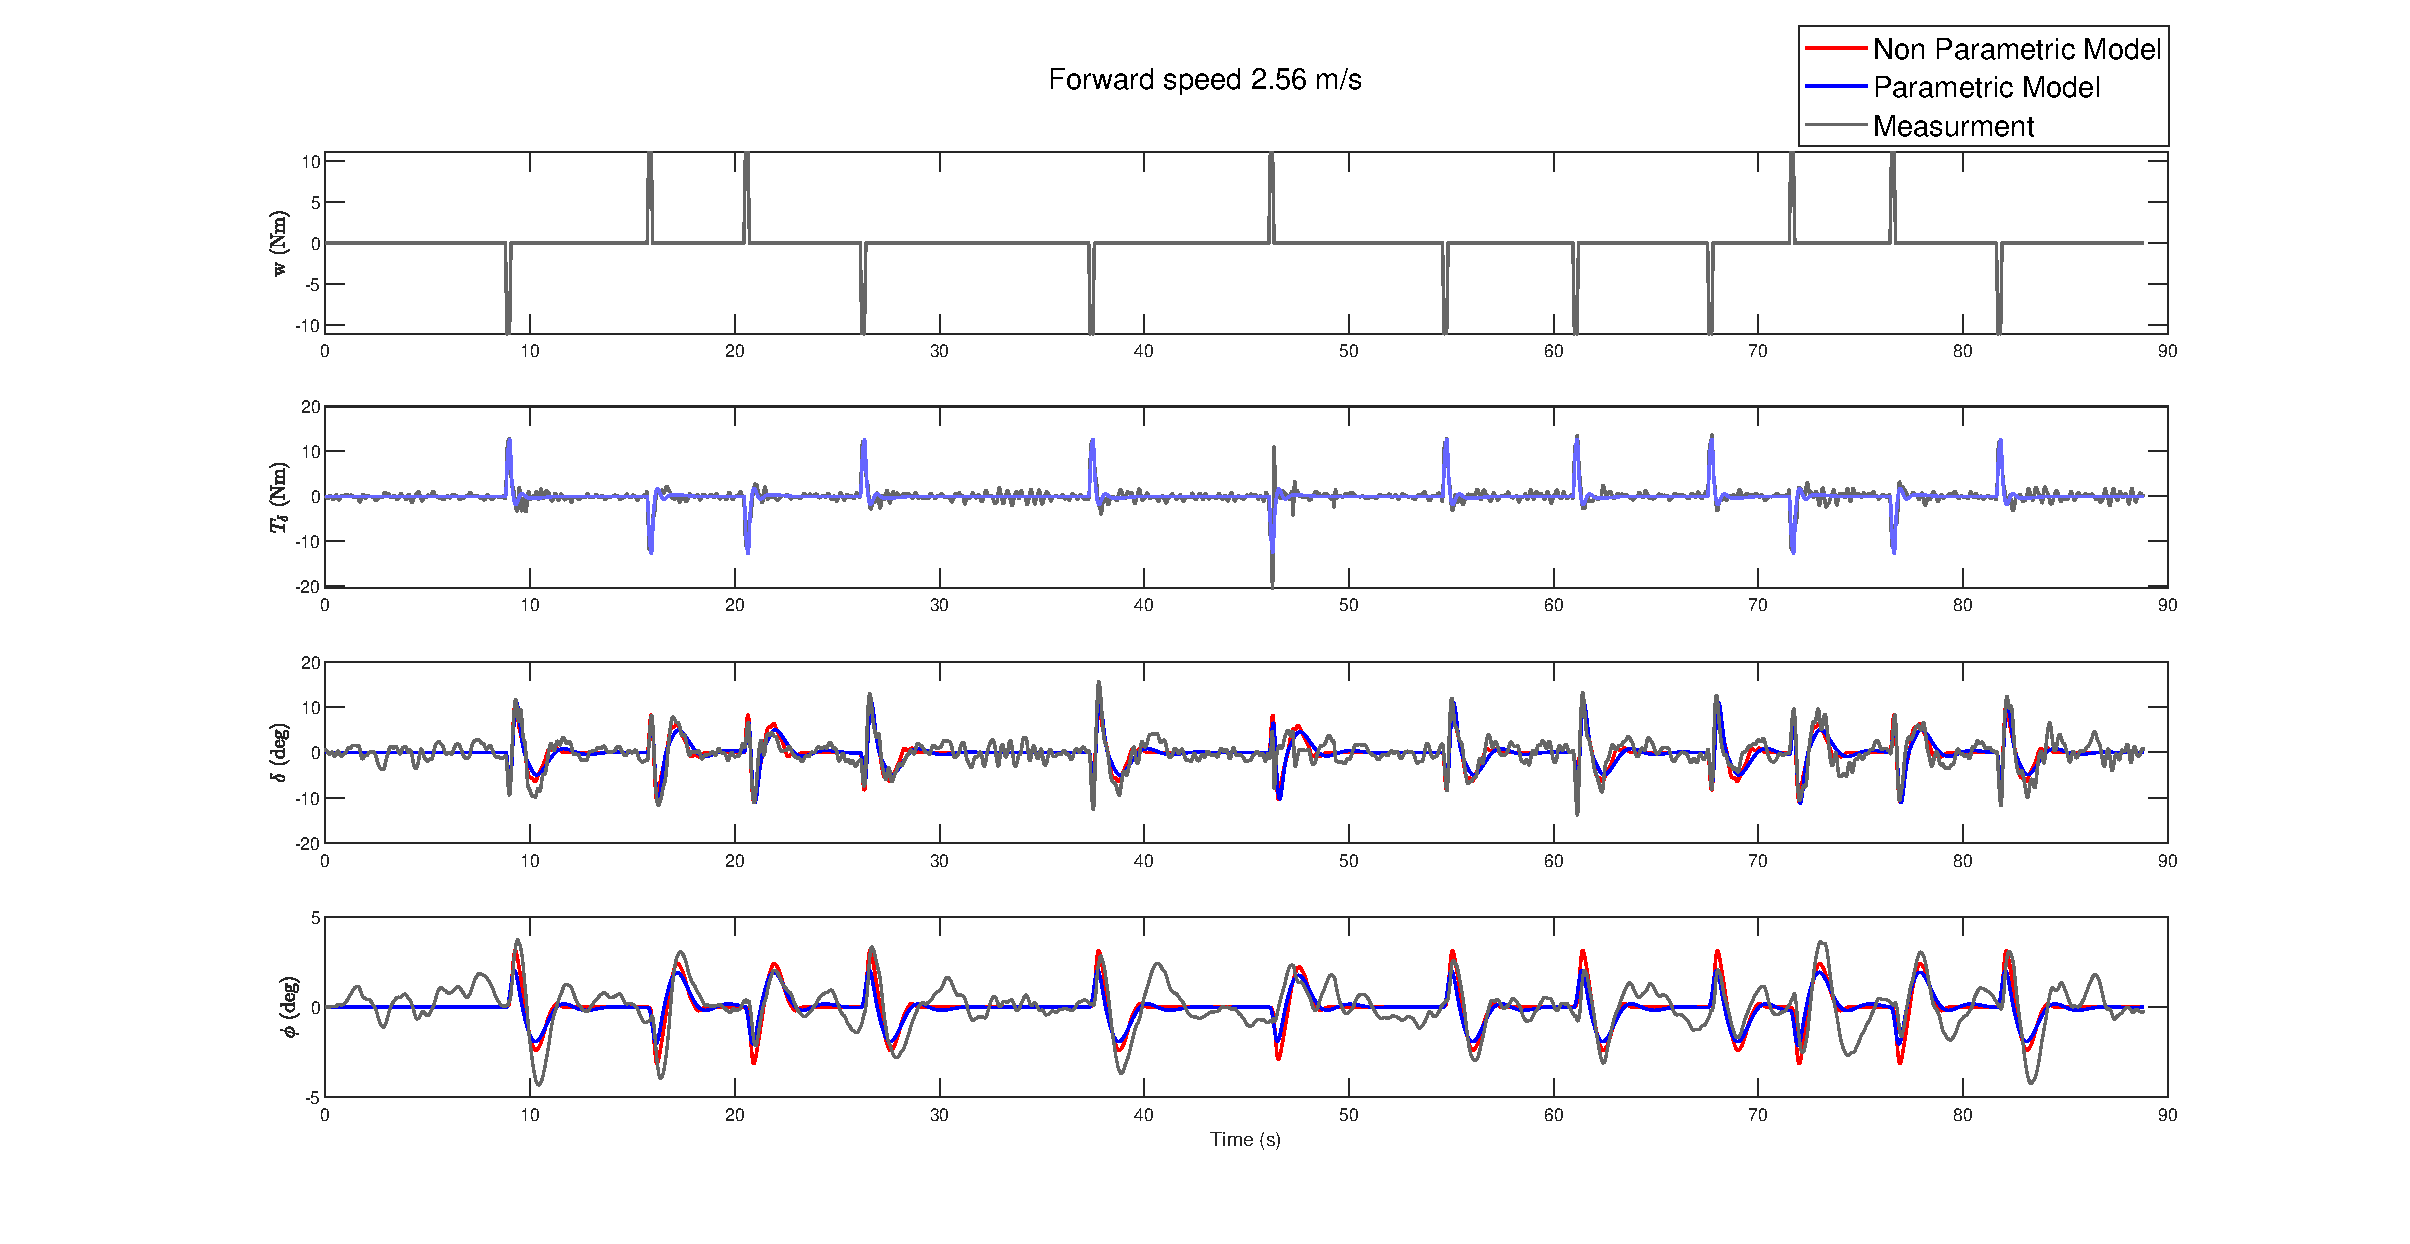
\includegraphics[width=1.4\linewidth]{images/steer_irf/param_signals_25.eps}}
        \caption{}
        \label{fig:model1}
    \end{subfigure}
    \begin{subfigure}[b]{\textwidth}
        \centering
        \makebox[\textwidth][c]{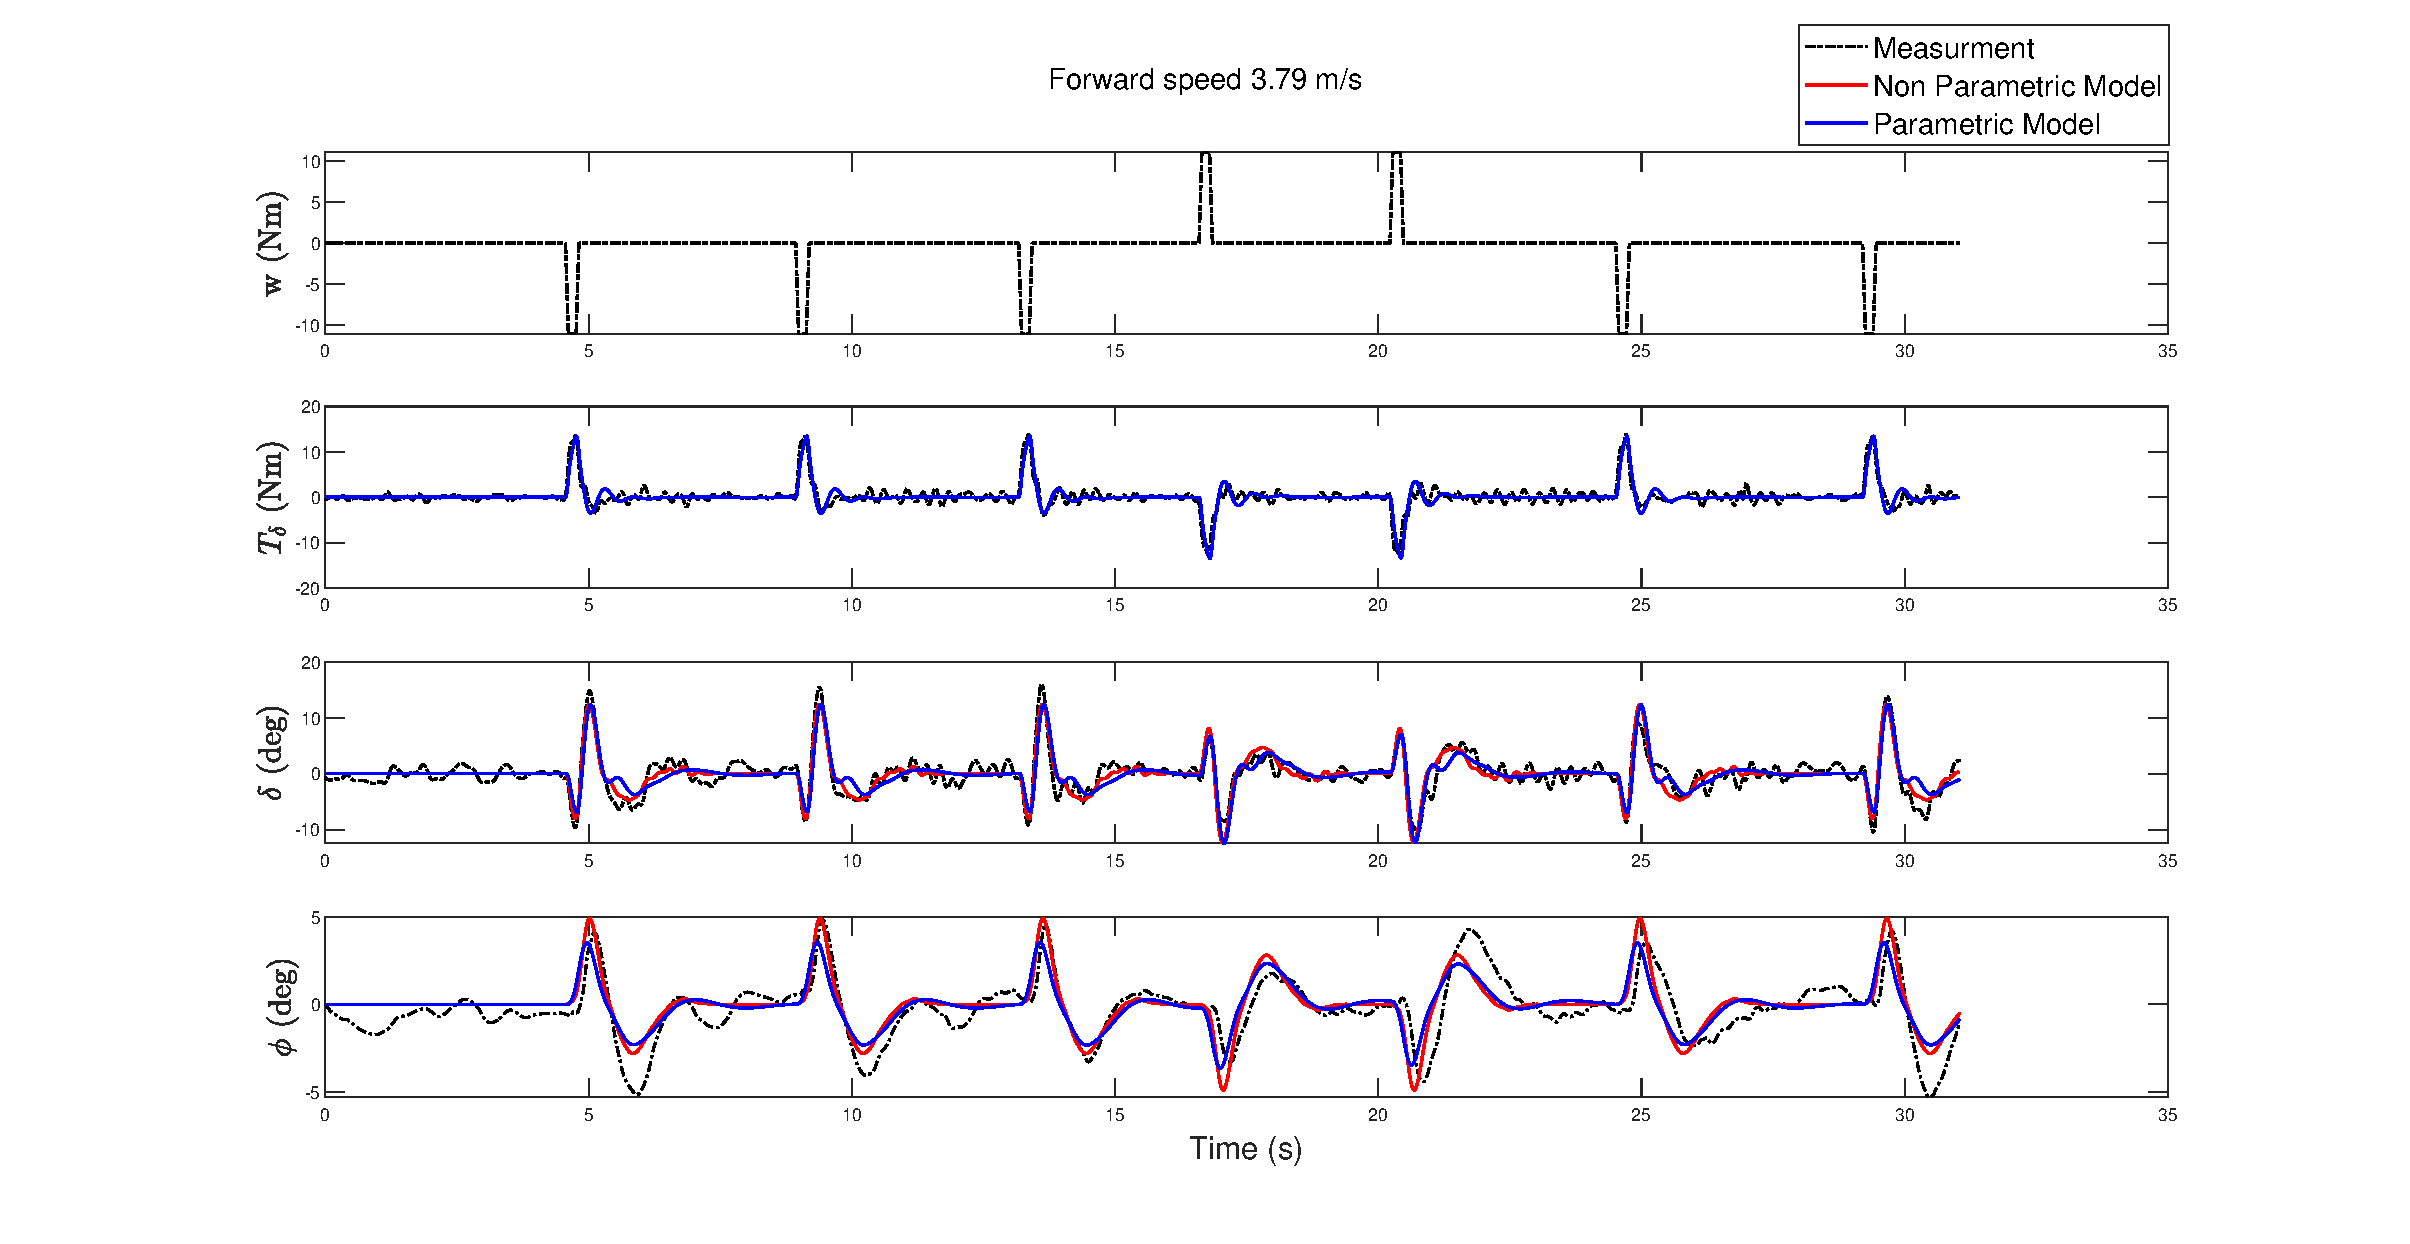
\includegraphics[width=1.4\linewidth]{images/steer_irf/param_signals_38.eps}}
        \caption{}            
        \label{fig:model2}
    \end{subfigure}
    \caption{Comparison between parametric model output, non-parametric model ouput and measured signals for the two lowest speed levels for the first participant.}
    \label{fig:model12}
 \end{figure}
 \begin{figure}
    \centering
    \begin{subfigure}[b]{\textwidth}
        \centering
        \makebox[\textwidth][c]{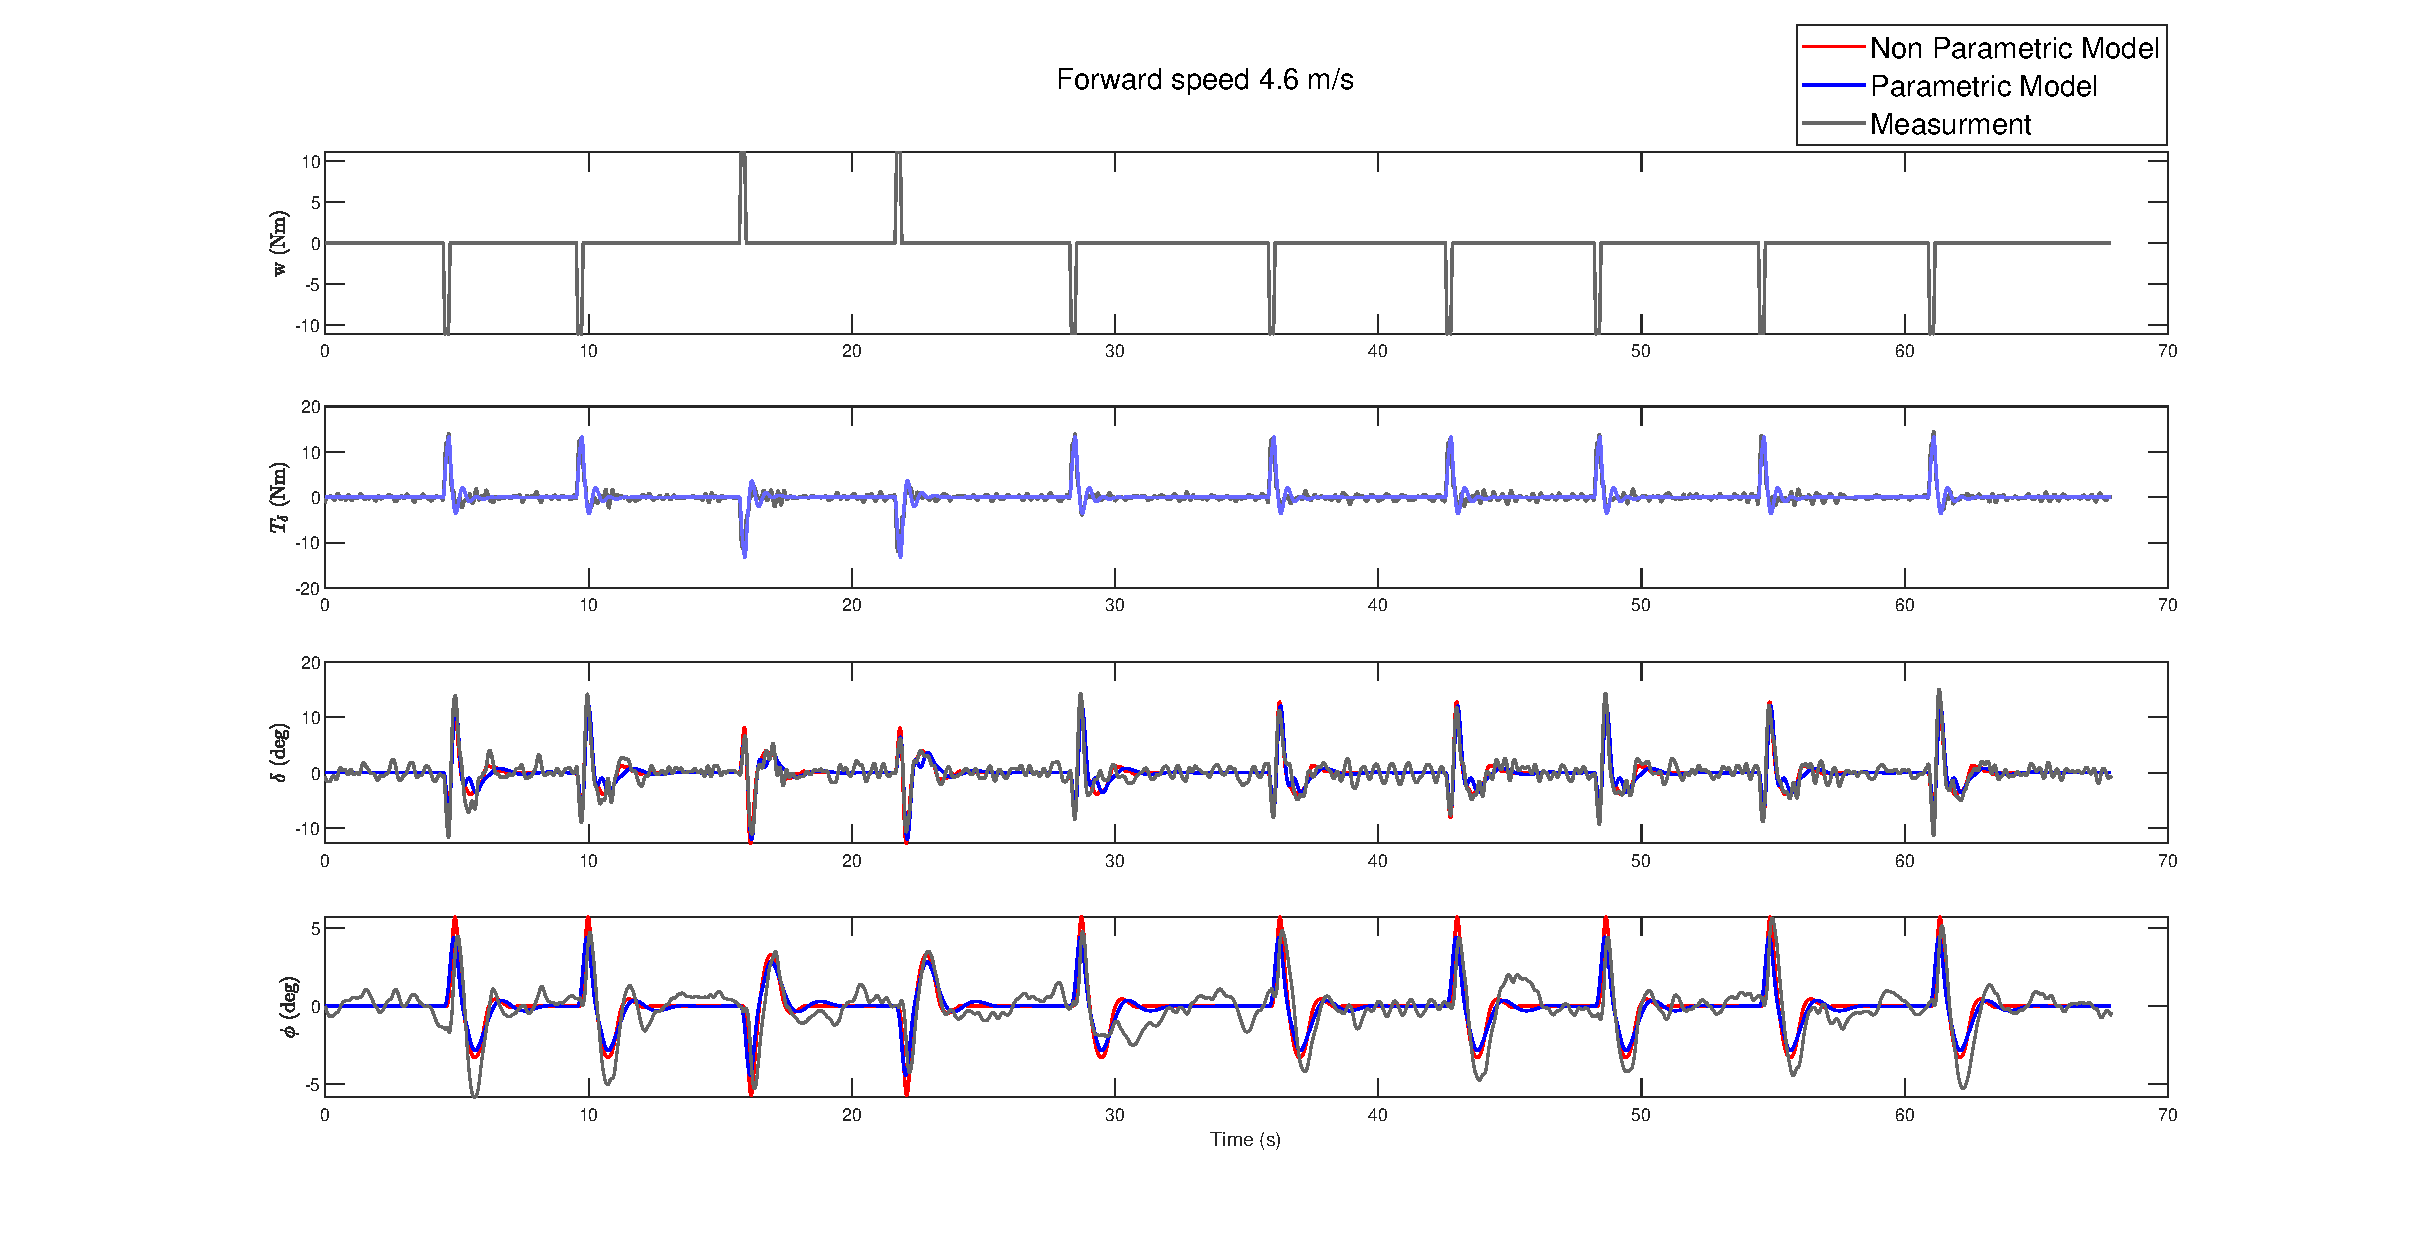
\includegraphics[width=1.4\linewidth]{images/steer_irf/param_signals_46.eps}}
        \caption{}
        \label{fig:model3}
    \end{subfigure}
    \begin{subfigure}[b]{\textwidth}
        \centering
        \makebox[\textwidth][c]{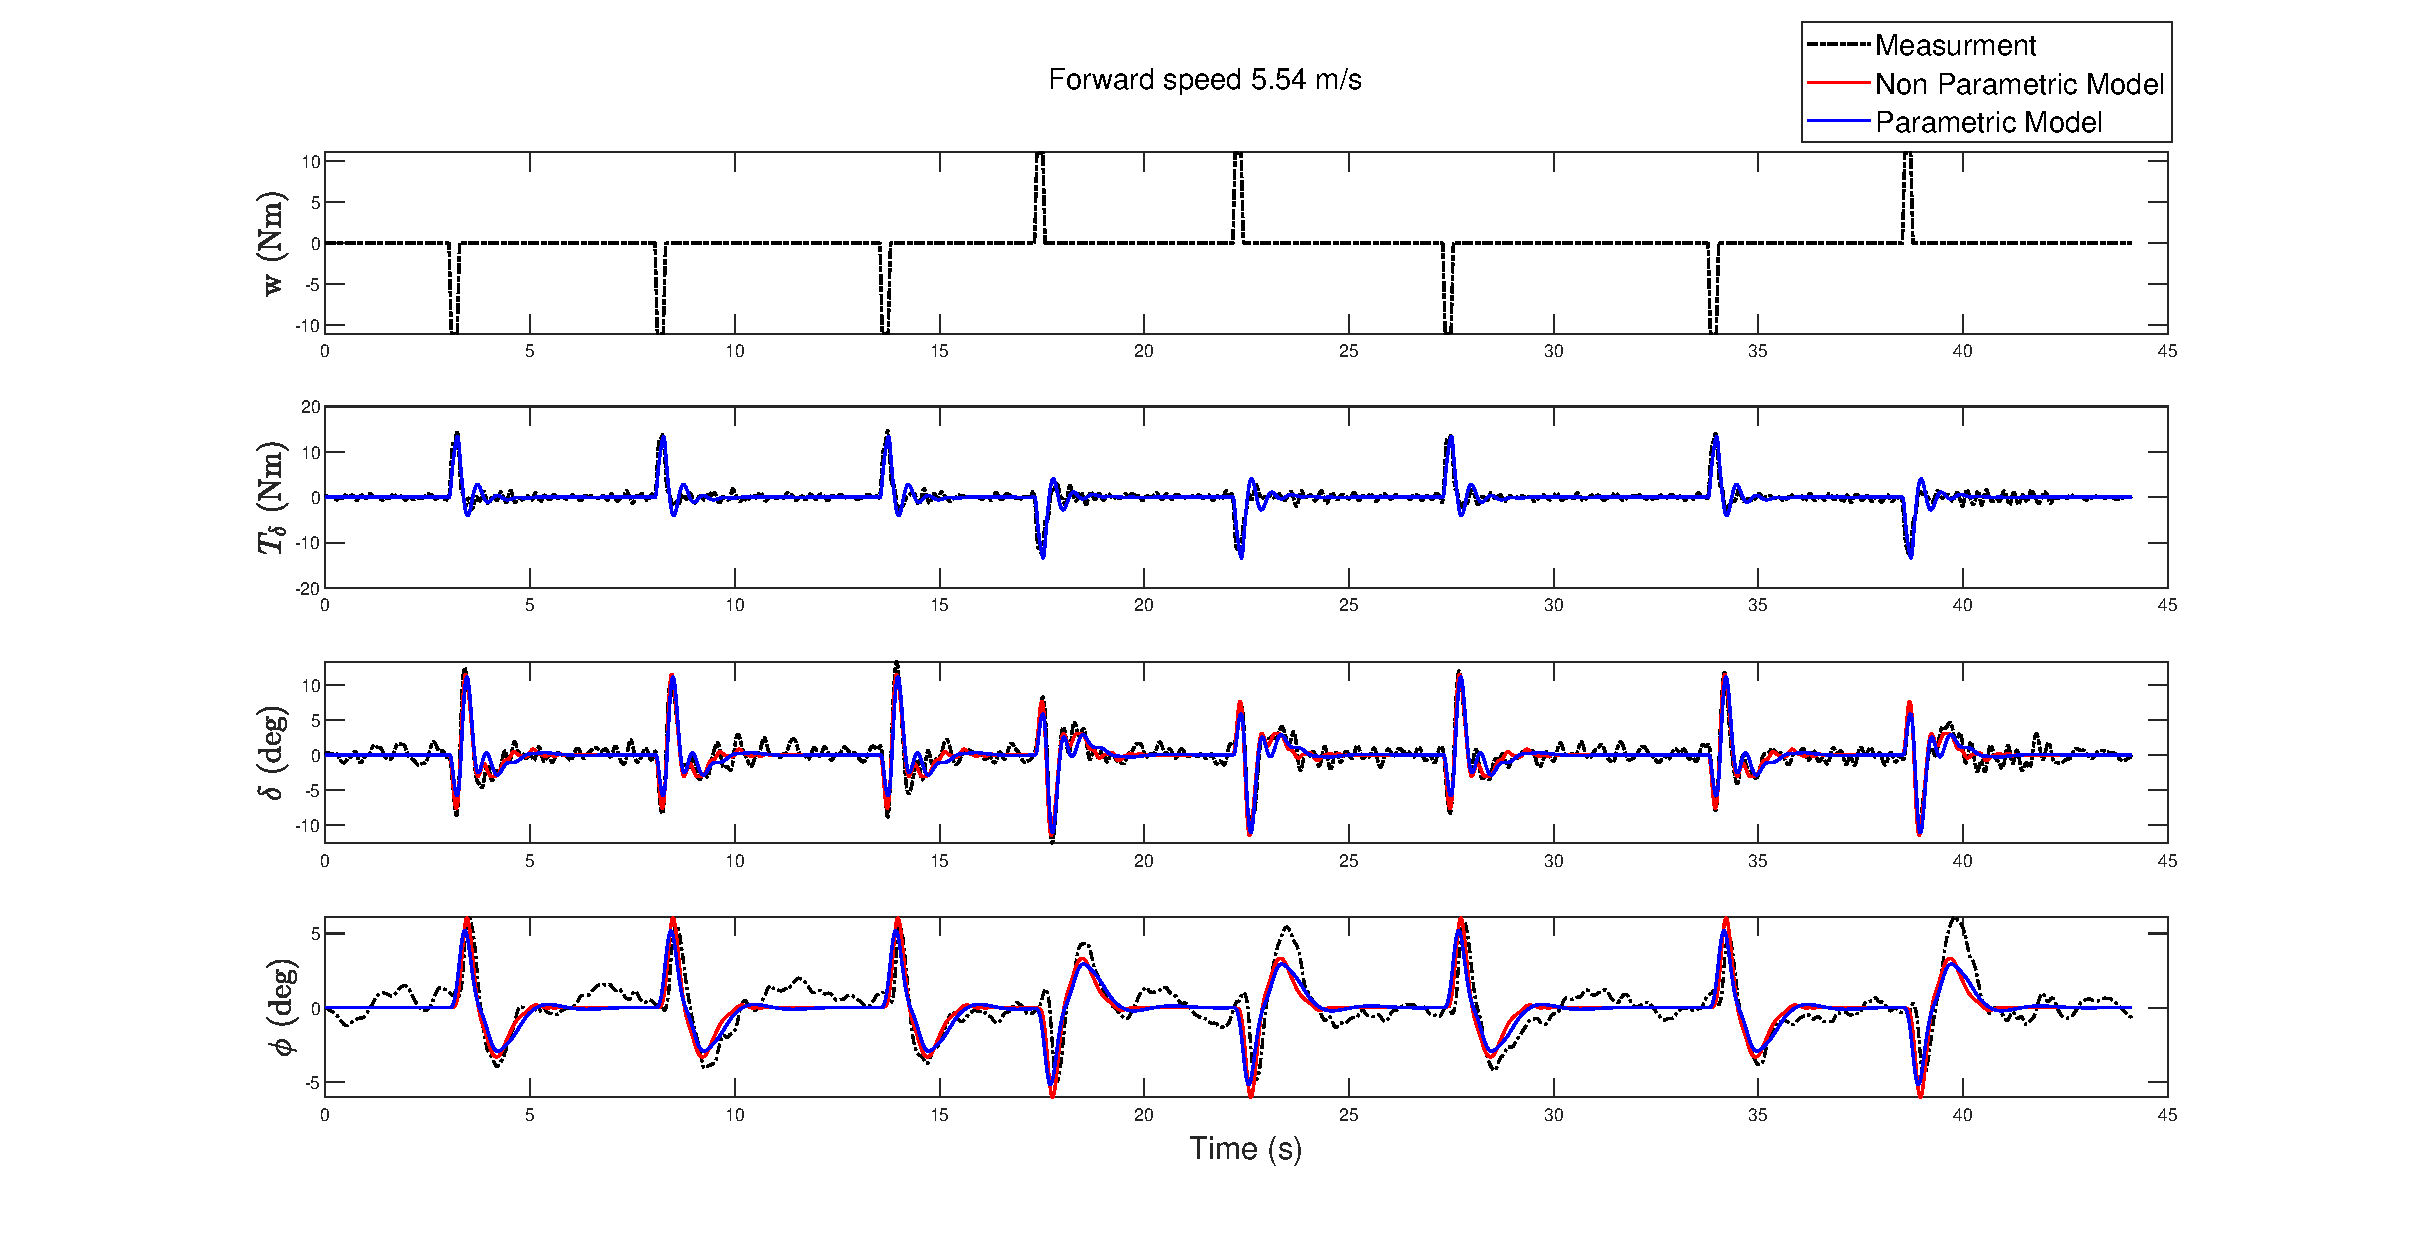
\includegraphics[width=1.4\linewidth]{images/steer_irf/param_signals_55.eps}}
        \caption{}            
        \label{fig:model4}
    \end{subfigure}
    \caption{Comparison between parametric model output, non-parametric model ouput and measured signals for the two highest speed levels for the first participant.}
    \label{fig:model34}
 \end{figure}

 \begin{figure}[h!]
    \centering
    % \captionsetup{justification=centering,margin=2cm}

    \includegraphics[width=\linewidth]{images/steer_irf/param_fit_box.eps}
    \caption{Box plot of the  \ensuremath{\mathrm{VAF}} between non-parametric output  of \ensuremath{\delta} (right) and \ensuremath{\phi} (left) and  parametric outputs \ensuremath{\hat{y}^\delta} and \ensuremath{\hat{y}^\phi}  for all forward speed levels.}
    \label{fig:FIT_model}
\end{figure}
The seven gains estimated for all participants are shown in \cref{fig:gain_plots_steer,tb:steer_gains}. Approximate linear trends are noted for all gains. Additionally, the intersubject variability for the forward speed level of 2.6 \si{\meter\per\second} is disproportionally higher than the rest, as noted by the much larger standard deviation in all gains. In \cref{fig:param_input} the decomposition of the input signal as the rider responds to the first perturbation of each forward speed level's run is shown. The intrinsic torque \ensuremath{T_\delta^{int}} initially acts as expected countering part of the perturbation torque, after that however it acts as a  regulatory mechanism, mirroring the reflexive response.

    \begin{table}[]
        \caption{Mean and standard deviation of all controller gains as estimated for the 14 participants.}
        \resizebox{\columnwidth}{!}{%
        \begin{tabular}{lllllllllllllll}
        $v\;\;\;(\si{m.s^{-1}})$                       & \multicolumn{2}{l}{$K_{\dot{\phi}}\;\;\;\;(\si{kg.m^2.s^{-2}})$} & \multicolumn{2}{l}{$K_{\dot{\delta}}\;\;\;\;(\si{kg.m^2.s^{-2}})$} & \multicolumn{2}{l}{$K_{{\phi}}\;\;\;\;(\si{kg.m^2.s^{-1}})$} & \multicolumn{2}{l}{$K^{ref}_{{\delta}}\;\;\;\;(\si{kg.m^2.s^{-1}})$} & \multicolumn{2}{l}{$K_{T_{\delta}}\;\;\;\;(-)$} & \multicolumn{2}{l}{$K^{ref}_{\dot{\delta}}\;\;\;\;(\si{kg.m^2.s^{-2}})$} & \multicolumn{2}{l}{$K^{int}_{{\delta}}\;\;\;\;(\si{kg.m^2.s^{-1}})$} \\ \cline{2-15} 
                                  & $\mu$                          & $\sigma$                        & $\mu$                          & $\sigma$                          & $\mu$                        & $\sigma$                      & $\mu$                           & $\sigma$                           & $\mu$                 & $\sigma$                & $\mu$                             & $\sigma$                             & $\mu$                           & $\sigma$                           \\ \hline
        \multicolumn{1}{l|}{2.68} & -55.10                         & 24.88                           & 1.66                           & 1.72                              & -89.90                       & 114.97                        & 6.60                            & 8.14                               & -0.99                 & 0.29                    & 10.14                             & 2.57                                 & 25.89                           & 24.41                              \\
        \multicolumn{1}{l|}{3.68} & -37.16                         & 12.15                           & 3.81                           & 2.04                              & -48.48                       & 14.75                         & 8.82                            & 8.94                               & -1.04                 & 0.05                    & 9.54                              & 2.72                                 & 30.19                           & 9.36                               \\
        \multicolumn{1}{l|}{4.49} & -29.57                         & 8.52                            & 4.27                           & 1.25                              & -43.72                       & 17.69                         & 12.13                           & 11.47                              & -1.02                 & 0.08                    & 8.97                              & 2.61                                 & 39.82                           & 14.24                              \\
        \multicolumn{1}{l|}{5.63} & -23.72                         & 7.26                            & 5.67                           & 2.51                              & -37.68                       & 16.46                         & 13.40                           & 14.29                              & -1.00                 & 0.08                    & 7.79                              & 2.47                                 & 52.89                           & 15.44                             
        \end{tabular}%
        }
        \label{tb:steer_gains}
        \end{table}
\begin{figure}[h!]
    \centering
    % \captionsetup{justification=centering,margin=2cm}

    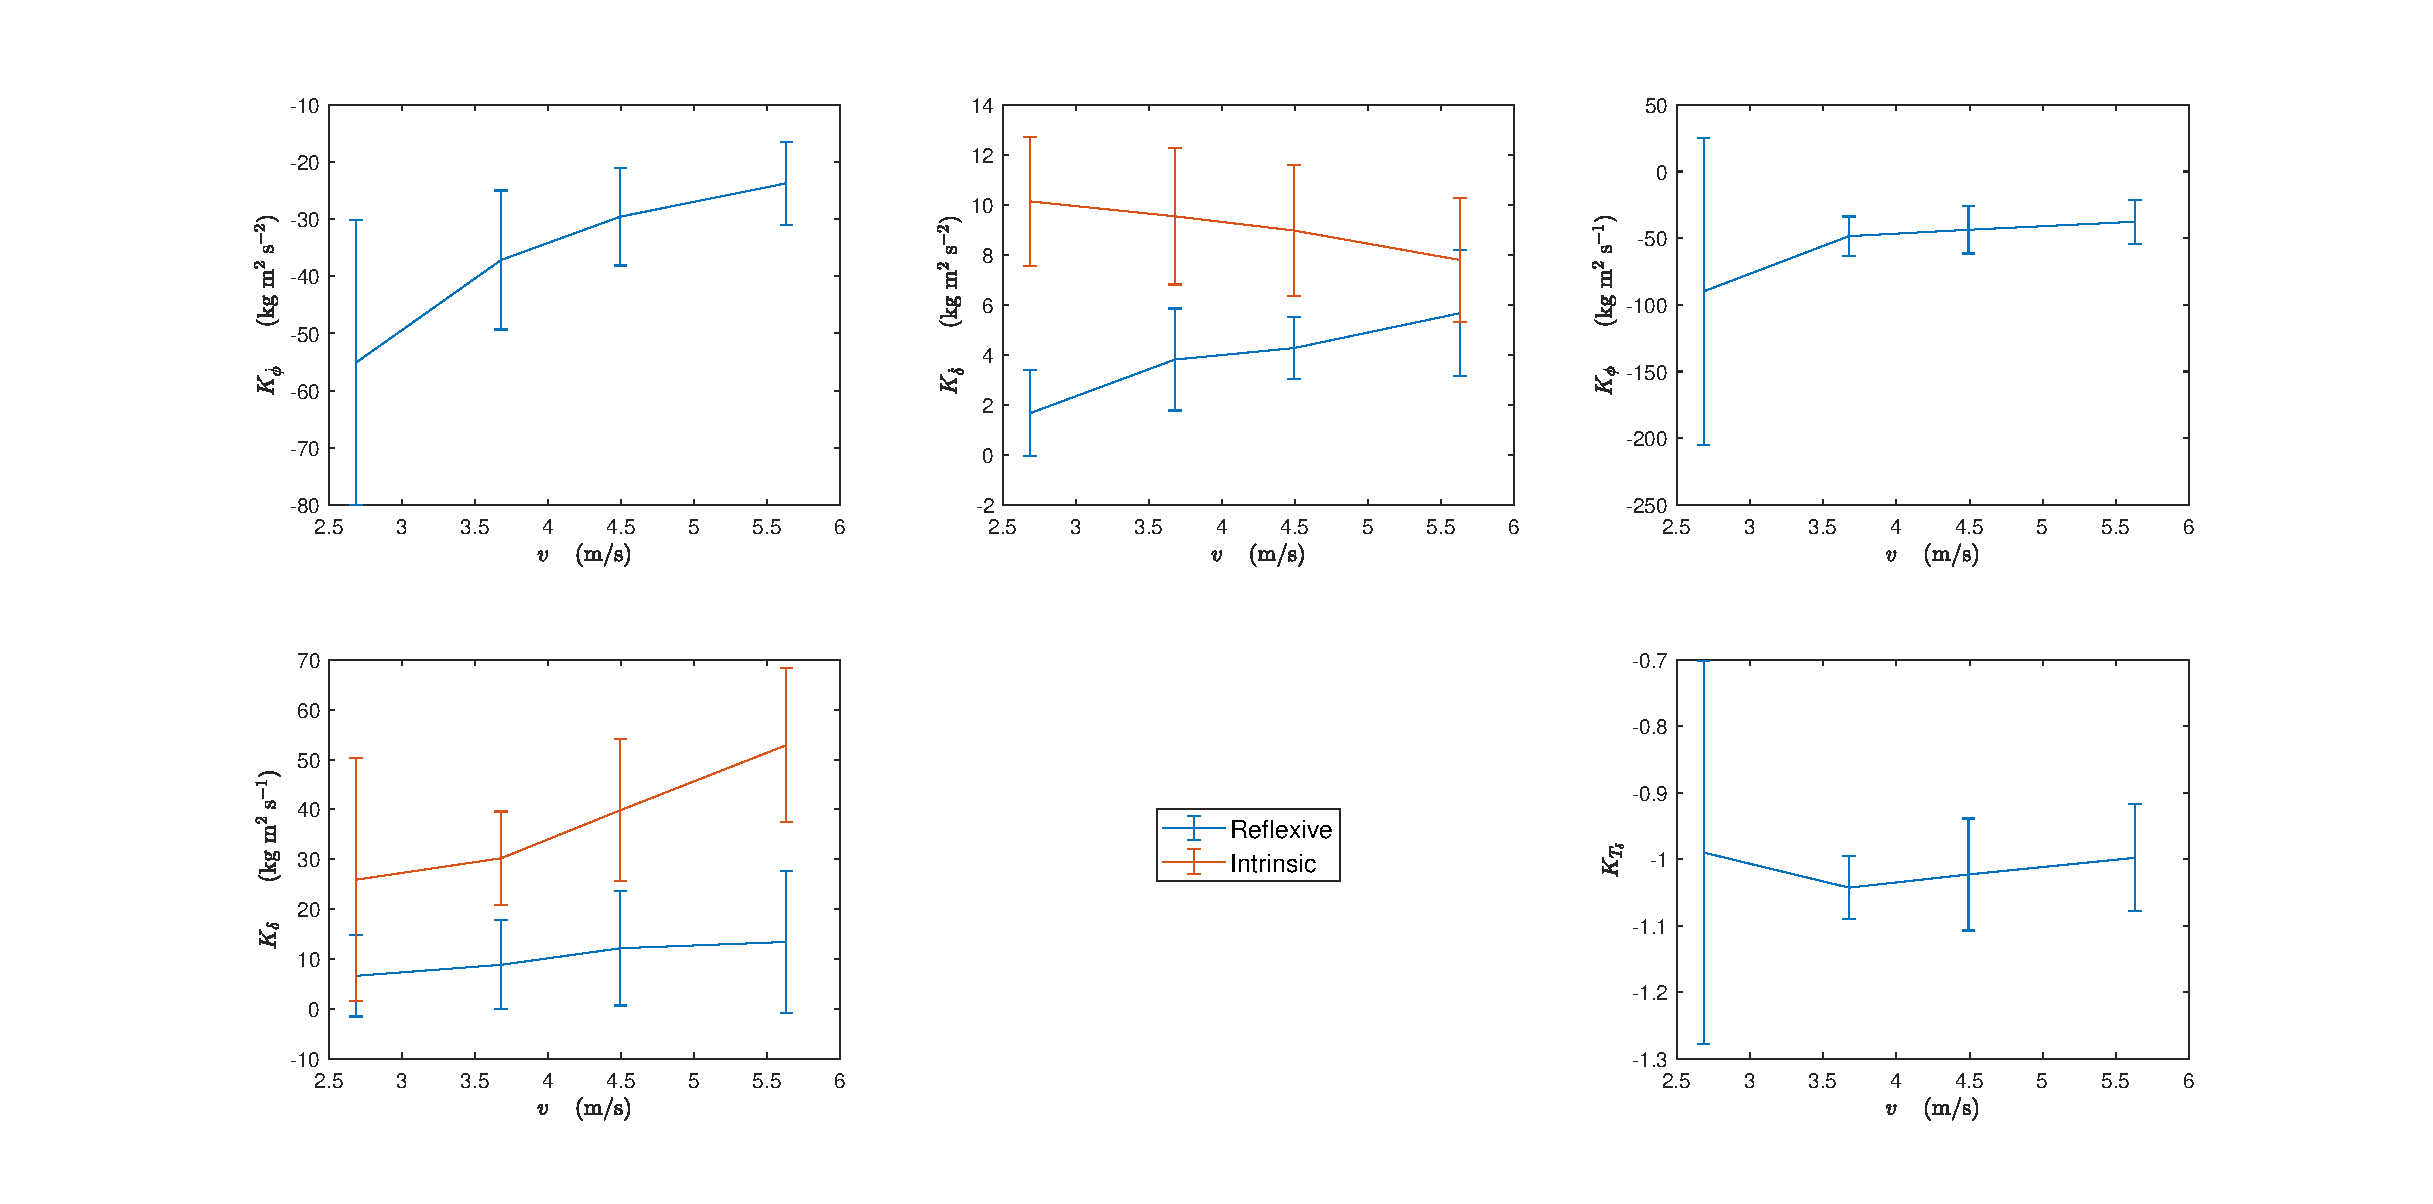
\includegraphics[width=\linewidth]{images/steer_irf/param_gains_plot.eps}
    \caption{Mean of estimated gains as a function of forward speed. Error bars indicate one standard deviation of the mean.}
    \label{fig:gain_plots_steer}
\end{figure}

\begin{figure}[h!]
    \centering
    % \captionsetup{justification=centering,margin=2cm}

    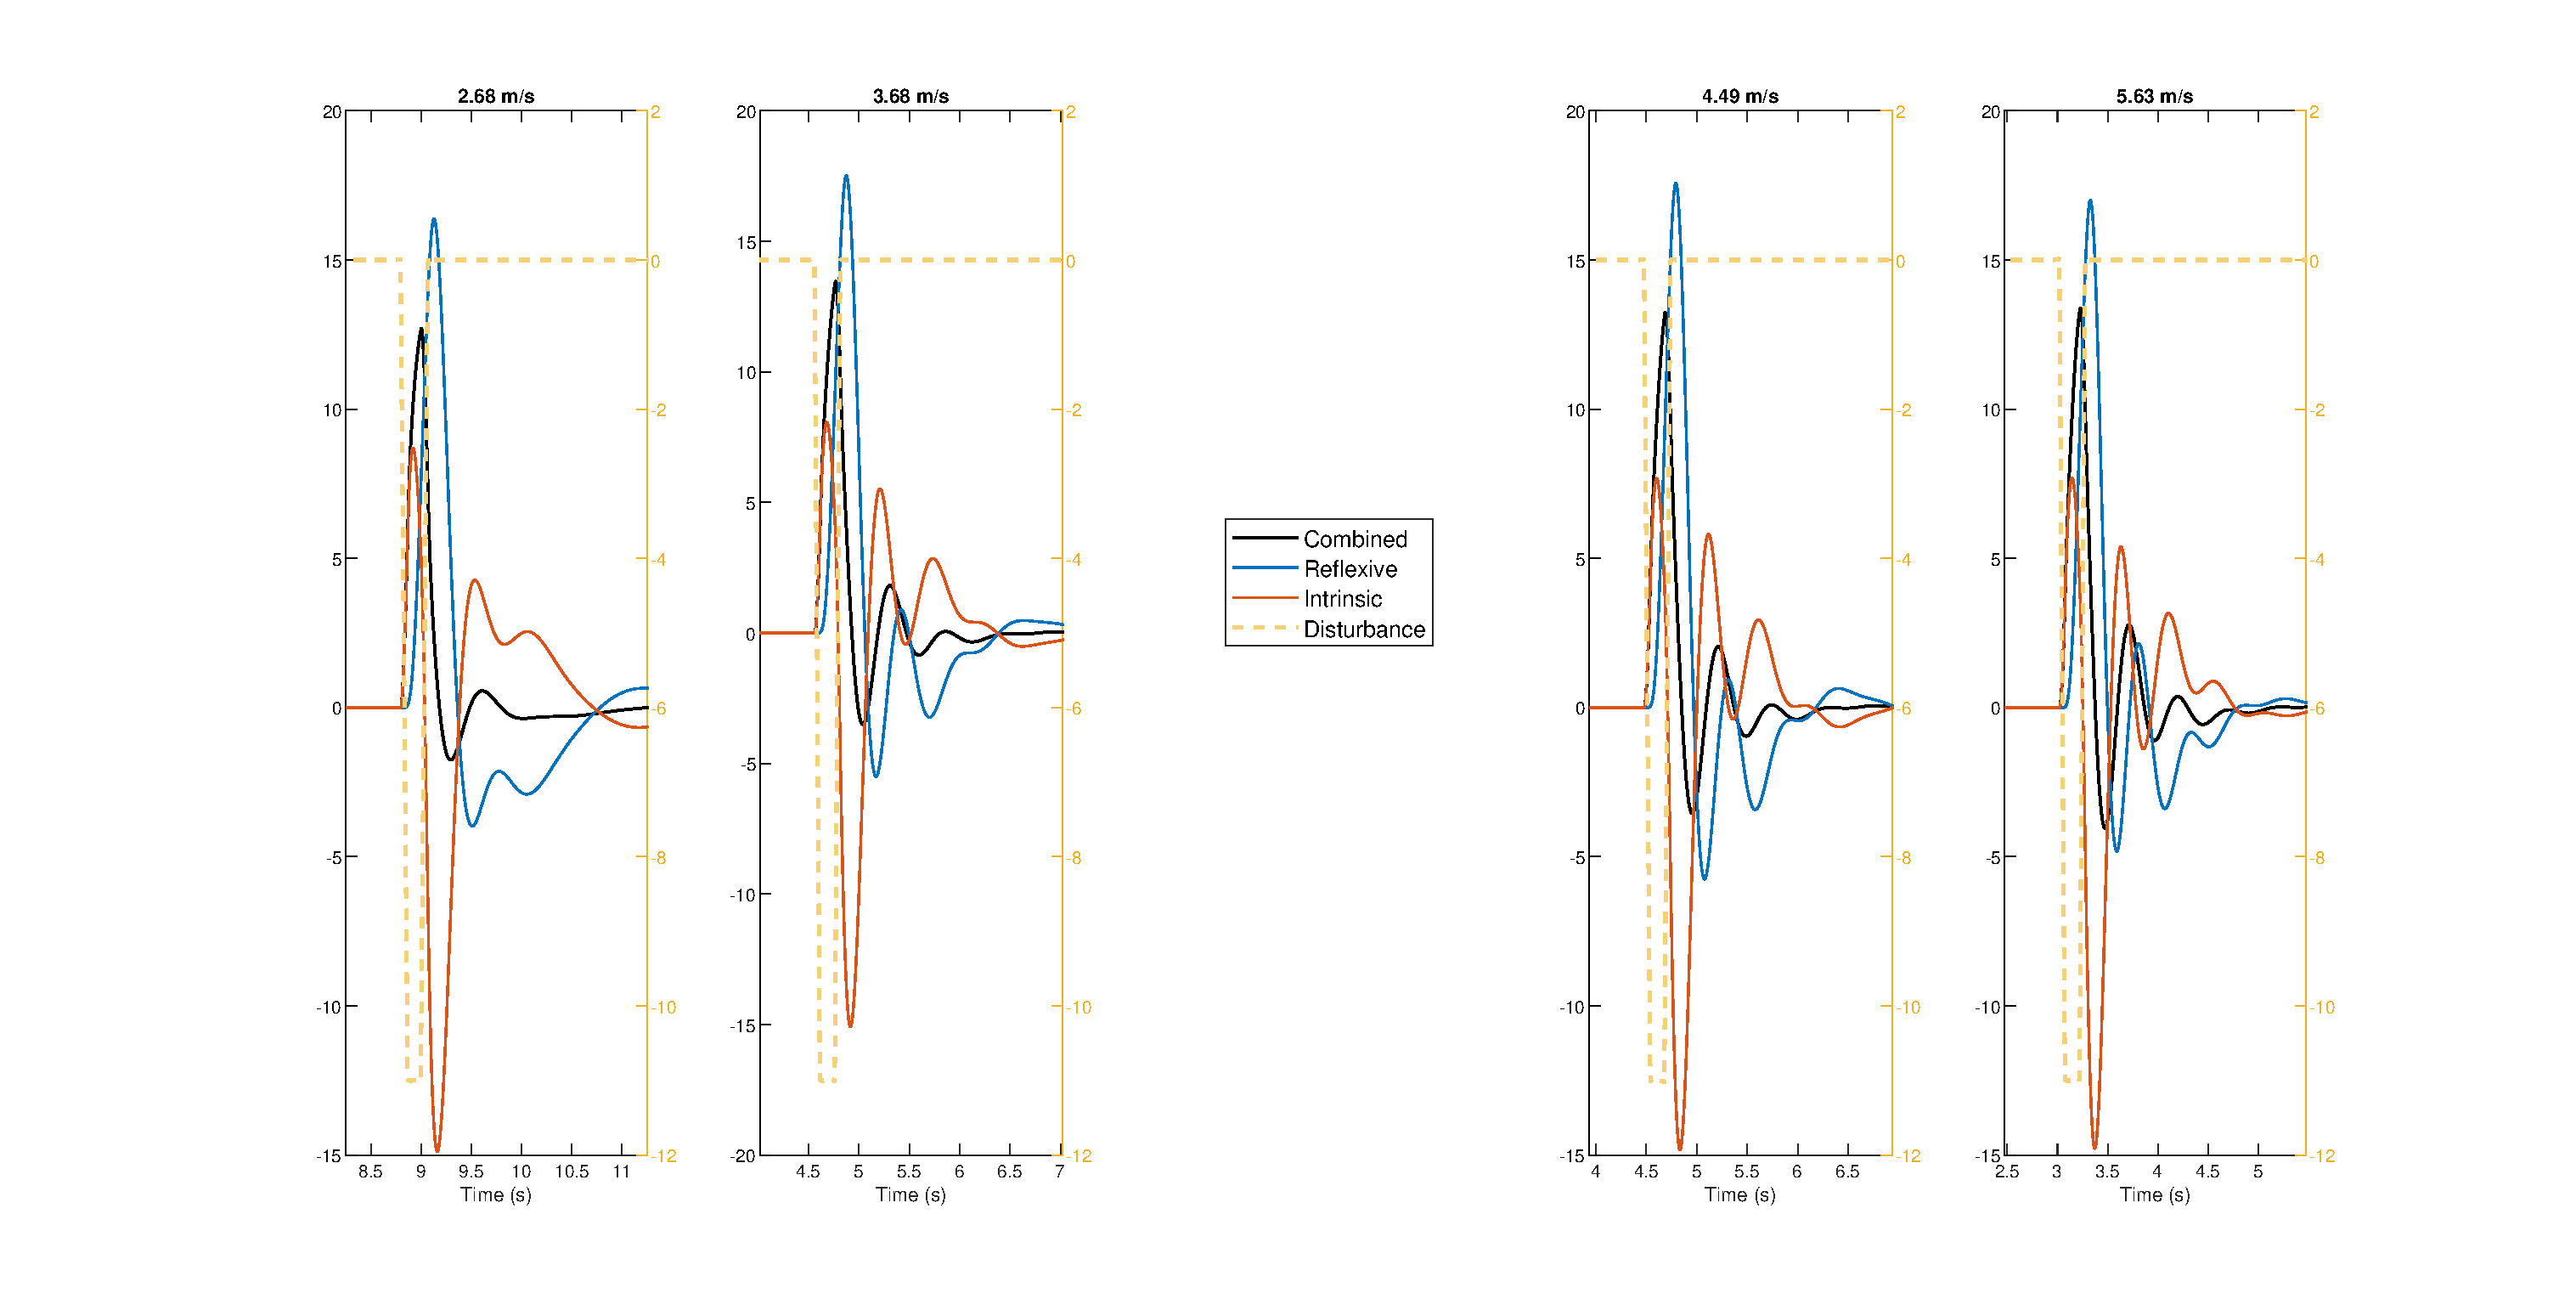
\includegraphics[width=\linewidth]{images/steer_irf/param_input.eps}
    \caption{Steering torque response to the first perturbation (dashed yellow) of the first participant as a function of time. The input is decomposed in the intrinsic component(orange) and the reflexive component (blue). }
    \label{fig:param_input}
\end{figure}
\section{Discussion}
As seen by \cref{fig:FIT_FIR} the \ensuremath{\mathrm{VAF}} is relatively low especially for roll angle \ensuremath{\phi} which means that significant variations in rider response within the same trial are present. This shows that the participants adapted their strategies as the trial went forward, consciously choosing to be more compliant or stiff depending on the situation. Despite the fact the experimental procedure was conducted in a much more proper manner than in the lateral perturbation experiment, meaning that subjects could in no way expect the bilateral perturbations sent through the wireless interface, the nature of the steering perturbation is such that allowed the participants to damp out big parts of the disturbance through cocontraction. One of the goals of this study is to investigate  the balance between reflexive response and cocontraction. However since we assume the bicycle to be linear time invariant for fixed forward speeds we expect consistent rider behavior as a function of speed, which means that the large intrasubject variability can not be captured by the model.

The lowest forward speed level displays disproportional level of variability as shown by the huge standard deviation margins across estimated parameters (see \cref{fig:gain_plots_steer}). This indicates that the intersubject variability present for that speed level is significantly higher. This could be an after effect of the the fact that the lowest speed level was always the first run. Although trial runs were conducted beforehand at various speed levels, some participants may not have adapted to the system completely which caused them to exhibit significant variance in their response.

Negative proportional and derivative gains for roll angle \ensuremath{\phi} indicate the reliance on the so called "steer into the fall" mechanism.   Modulation of steering stiffness is dominated by cocontraction as the reflexive \ensuremath{K_\delta} stays close to zero across speed levels (see \cref{fig:gain_plots_steer}). An increasing reliance on intrinsic steering stiffness as speed increases is noted. On the other hand, the intrinsic modulation of steering damping is lessened as speed increases, in favor of the reflexive pathway (see \cref{fig:gain_plots_steer}). What is more interesting however is the way the intrinsic and reflexive components of the control input interact with each other in order to create the final applied rider torque. The torque generated by cocontraction initially acts as a way to lessen the  impact of the perturbation as seen by the first few milliseconds in the intrinsic signal of \cref{fig:param_input}. During optimization of the parameters the intrinsic gains are tuned in order to best counter initial impact on the steering states by the perturbation. However since we assume a time invariant  system the same parameters act on the later milliseconds as well, creating the weird mirroring effect between reflexive and intrinsic components. This upon initial observation seems counter intuitive since it seems that the reflexive controller is fighting against the intrinsic one. The reason why this happens is the fact that the reflexive response is dominated by the "steer into the fall" strategy of control, while the intrinsic mechanism is trying to achieve  steering angles and rates equal to zero. In reality the intrinsic response of the rider is not time invariant. At the first few milliseconds of the perturbation cocontraction is active while afterwards when the rider needs to actually balance the bike by steering into the fall cocontraction is lessened and the reflexive is the main mechanism of control.  In a more realistic model this behavior should be captured.
\section{Conclusions}
In conclusion the rider model created manages to achieve a good level of fit and simultaneously captures the significance of the intrinsic response when countering steering torque perturbations. A high level of intersubject variability is exhibited. The hypothesis that this variability is in fact due to the modulation of admittance in the shoulder joint is strongly indicated. Despite all that,  the assumption that for constant speeds the system is time invariant does not seem to hold ground as noted by the irregular effect of cocontraction in the later stages of the rider  response.